\documentclass{ximera}

%\usepackage{todonotes}

\newcommand{\todo}{}

\usepackage{esint} % for \oiint
\ifxake%%https://math.meta.stackexchange.com/questions/9973/how-do-you-render-a-closed-surface-double-integral
\renewcommand{\oiint}{{\large\bigcirc}\kern-1.56em\iint}
\fi


\graphicspath{
  {./}
  {ximeraTutorial/}
  {basicPhilosophy/}
  {functionsOfSeveralVariables/}
  {normalVectors/}
  {lagrangeMultipliers/}
  {vectorFields/}
  {greensTheorem/}
  {shapeOfThingsToCome/}
  {dotProducts/}
  {partialDerivativesAndTheGradientVector/}
  {../productAndQuotientRules/exercises/}
  {../normalVectors/exercisesParametricPlots/}
  {../continuityOfFunctionsOfSeveralVariables/exercises/}
  {../partialDerivativesAndTheGradientVector/exercises/}
  {../directionalDerivativeAndChainRule/exercises/}
  {../commonCoordinates/exercisesCylindricalCoordinates/}
  {../commonCoordinates/exercisesSphericalCoordinates/}
  {../greensTheorem/exercisesCurlAndLineIntegrals/}
  {../greensTheorem/exercisesDivergenceAndLineIntegrals/}
  {../shapeOfThingsToCome/exercisesDivergenceTheorem/}
  {../greensTheorem/}
  {../shapeOfThingsToCome/}
  {../separableDifferentialEquations/exercises/}
  {vectorFields/}
}

\newcommand{\mooculus}{\textsf{\textbf{MOOC}\textnormal{\textsf{ULUS}}}}

\usepackage{tkz-euclide}
\usepackage{tikz}
\usepackage{tikz-cd}
\usetikzlibrary{arrows}
\tikzset{>=stealth,commutative diagrams/.cd,
  arrow style=tikz,diagrams={>=stealth}} %% cool arrow head
\tikzset{shorten <>/.style={ shorten >=#1, shorten <=#1 } } %% allows shorter vectors

\usetikzlibrary{backgrounds} %% for boxes around graphs
\usetikzlibrary{shapes,positioning}  %% Clouds and stars
\usetikzlibrary{matrix} %% for matrix
\usepgfplotslibrary{polar} %% for polar plots
\usepgfplotslibrary{fillbetween} %% to shade area between curves in TikZ
%\usetkzobj{all}
\usepackage[makeroom]{cancel} %% for strike outs
%\usepackage{mathtools} %% for pretty underbrace % Breaks Ximera
%\usepackage{multicol}
\usepackage{pgffor} %% required for integral for loops



%% http://tex.stackexchange.com/questions/66490/drawing-a-tikz-arc-specifying-the-center
%% Draws beach ball
\tikzset{pics/carc/.style args={#1:#2:#3}{code={\draw[pic actions] (#1:#3) arc(#1:#2:#3);}}}



\usepackage{array}
\setlength{\extrarowheight}{+.1cm}
\newdimen\digitwidth
\settowidth\digitwidth{9}
\def\divrule#1#2{
\noalign{\moveright#1\digitwidth
\vbox{\hrule width#2\digitwidth}}}




% \newcommand{\RR}{\mathbb R}
% \newcommand{\R}{\mathbb R}
% \newcommand{\N}{\mathbb N}
% \newcommand{\Z}{\mathbb Z}

\newcommand{\sagemath}{\textsf{SageMath}}


%\renewcommand{\d}{\,d\!}
%\renewcommand{\d}{\mathop{}\!d}
%\newcommand{\dd}[2][]{\frac{\d #1}{\d #2}}
%\newcommand{\pp}[2][]{\frac{\partial #1}{\partial #2}}
% \renewcommand{\l}{\ell}
%\newcommand{\ddx}{\frac{d}{\d x}}

% \newcommand{\zeroOverZero}{\ensuremath{\boldsymbol{\tfrac{0}{0}}}}
%\newcommand{\inftyOverInfty}{\ensuremath{\boldsymbol{\tfrac{\infty}{\infty}}}}
%\newcommand{\zeroOverInfty}{\ensuremath{\boldsymbol{\tfrac{0}{\infty}}}}
%\newcommand{\zeroTimesInfty}{\ensuremath{\small\boldsymbol{0\cdot \infty}}}
%\newcommand{\inftyMinusInfty}{\ensuremath{\small\boldsymbol{\infty - \infty}}}
%\newcommand{\oneToInfty}{\ensuremath{\boldsymbol{1^\infty}}}
%\newcommand{\zeroToZero}{\ensuremath{\boldsymbol{0^0}}}
%\newcommand{\inftyToZero}{\ensuremath{\boldsymbol{\infty^0}}}



% \newcommand{\numOverZero}{\ensuremath{\boldsymbol{\tfrac{\#}{0}}}}
% \newcommand{\dfn}{\textbf}
% \newcommand{\unit}{\,\mathrm}
% \newcommand{\unit}{\mathop{}\!\mathrm}
% \newcommand{\eval}[1]{\bigg[ #1 \bigg]}
% \newcommand{\seq}[1]{\left( #1 \right)}
% \renewcommand{\epsilon}{\varepsilon}
% \renewcommand{\phi}{\varphi}


% \renewcommand{\iff}{\Leftrightarrow}

% \DeclareMathOperator{\arccot}{arccot}
% \DeclareMathOperator{\arcsec}{arcsec}
% \DeclareMathOperator{\arccsc}{arccsc}
% \DeclareMathOperator{\si}{Si}
% \DeclareMathOperator{\scal}{scal}
% \DeclareMathOperator{\sign}{sign}


%% \newcommand{\tightoverset}[2]{% for arrow vec
%%   \mathop{#2}\limits^{\vbox to -.5ex{\kern-0.75ex\hbox{$#1$}\vss}}}
% \newcommand{\arrowvec}[1]{{\overset{\rightharpoonup}{#1}}}
% \renewcommand{\vec}[1]{\arrowvec{\mathbf{#1}}}
% \renewcommand{\vec}[1]{{\overset{\boldsymbol{\rightharpoonup}}{\mathbf{#1}}}}

% \newcommand{\point}[1]{\left(#1\right)} %this allows \vector{ to be changed to \vector{ with a quick find and replace
% \newcommand{\pt}[1]{\mathbf{#1}} %this allows \vec{ to be changed to \vec{ with a quick find and replace
% \newcommand{\Lim}[2]{\lim_{\point{#1} \to \point{#2}}} %Bart, I changed this to point since I want to use it.  It runs through both of the exercise and exerciseE files in limits section, which is why it was in each document to start with.

% \DeclareMathOperator{\proj}{\mathbf{proj}}
% \newcommand{\veci}{{\boldsymbol{\hat{\imath}}}}
% \newcommand{\vecj}{{\boldsymbol{\hat{\jmath}}}}
% \newcommand{\veck}{{\boldsymbol{\hat{k}}}}
% \newcommand{\vecl}{\vec{\boldsymbol{\l}}}
% \newcommand{\uvec}[1]{\mathbf{\hat{#1}}}
% \newcommand{\utan}{\mathbf{\hat{t}}}
% \newcommand{\unormal}{\mathbf{\hat{n}}}
% \newcommand{\ubinormal}{\mathbf{\hat{b}}}

% \newcommand{\dotp}{\bullet}
% \newcommand{\cross}{\boldsymbol\times}
% \newcommand{\grad}{\boldsymbol\nabla}
% \newcommand{\divergence}{\grad\dotp}
% \newcommand{\curl}{\grad\cross}
%\DeclareMathOperator{\divergence}{divergence}
%\DeclareMathOperator{\curl}[1]{\grad\cross #1}
% \newcommand{\lto}{\mathop{\longrightarrow\,}\limits}

% \renewcommand{\bar}{\overline}

\colorlet{textColor}{black}
\colorlet{background}{white}
\colorlet{penColor}{blue!50!black} % Color of a curve in a plot
\colorlet{penColor2}{red!50!black}% Color of a curve in a plot
\colorlet{penColor3}{red!50!blue} % Color of a curve in a plot
\colorlet{penColor4}{green!50!black} % Color of a curve in a plot
\colorlet{penColor5}{orange!80!black} % Color of a curve in a plot
\colorlet{penColor6}{yellow!70!black} % Color of a curve in a plot
\colorlet{fill1}{penColor!20} % Color of fill in a plot
\colorlet{fill2}{penColor2!20} % Color of fill in a plot
\colorlet{fillp}{fill1} % Color of positive area
\colorlet{filln}{penColor2!20} % Color of negative area
\colorlet{fill3}{penColor3!20} % Fill
\colorlet{fill4}{penColor4!20} % Fill
\colorlet{fill5}{penColor5!20} % Fill
\colorlet{gridColor}{gray!50} % Color of grid in a plot

\newcommand{\surfaceColor}{violet}
\newcommand{\surfaceColorTwo}{redyellow}
\newcommand{\sliceColor}{greenyellow}




\pgfmathdeclarefunction{gauss}{2}{% gives gaussian
  \pgfmathparse{1/(#2*sqrt(2*pi))*exp(-((x-#1)^2)/(2*#2^2))}%
}


%%%%%%%%%%%%%
%% Vectors
%%%%%%%%%%%%%

%% Simple horiz vectors
\renewcommand{\vector}[1]{\left\langle #1\right\rangle}


%% %% Complex Horiz Vectors with angle brackets
%% \makeatletter
%% \renewcommand{\vector}[2][ , ]{\left\langle%
%%   \def\nextitem{\def\nextitem{#1}}%
%%   \@for \el:=#2\do{\nextitem\el}\right\rangle%
%% }
%% \makeatother

%% %% Vertical Vectors
%% \def\vector#1{\begin{bmatrix}\vecListA#1,,\end{bmatrix}}
%% \def\vecListA#1,{\if,#1,\else #1\cr \expandafter \vecListA \fi}

%%%%%%%%%%%%%
%% End of vectors
%%%%%%%%%%%%%

%\newcommand{\fullwidth}{}
%\newcommand{\normalwidth}{}



%% makes a snazzy t-chart for evaluating functions
%\newenvironment{tchart}{\rowcolors{2}{}{background!90!textColor}\array}{\endarray}

%%This is to help with formatting on future title pages.
\newenvironment{sectionOutcomes}{}{}



%% Flowchart stuff
%\tikzstyle{startstop} = [rectangle, rounded corners, minimum width=3cm, minimum height=1cm,text centered, draw=black]
%\tikzstyle{question} = [rectangle, minimum width=3cm, minimum height=1cm, text centered, draw=black]
%\tikzstyle{decision} = [trapezium, trapezium left angle=70, trapezium right angle=110, minimum width=3cm, minimum height=1cm, text centered, draw=black]
%\tikzstyle{question} = [rectangle, rounded corners, minimum width=3cm, minimum height=1cm,text centered, draw=black]
%\tikzstyle{process} = [rectangle, minimum width=3cm, minimum height=1cm, text centered, draw=black]
%\tikzstyle{decision} = [trapezium, trapezium left angle=70, trapezium right angle=110, minimum width=3cm, minimum height=1cm, text centered, draw=black]


\title{Refining}

\begin{document}

\begin{abstract}
open interval
\end{abstract}
\maketitle



Everything gets more complicated the deeper you look. \\


Mathematics is no different. \\


We are just getting started with the derivative and the more we examine it, the more complicated it will become. \\

We are ready for the next layer to this story. \\




\subsection*{So far...}


Our definition of the derivative has been a graphical definition.

\begin{idea}

Let $f(x)$ be a function with domain $D$. \\
Let $a \in D$ be a domain number. \\

Then $f(x)$ has a graph. \\

There are two possibilities:  \\


\textbf{\textcolor{blue!55!black}{1)}} \textbf{the graph has a tangent line at $(a, f(a))$}

\textbf{\textcolor{blue!55!black}{2)}} \textbf{the graph does not have a tangent line at $(a, f(a))$}




If the graph has a tangent line at $(a, f(a))$ and this tangent line has a slope, then


\begin{center}

$f'(a)$ = the slope of the tangent line at $(a, f(a))$,

\end{center}



Otherwise, we say that $f'(a)$ does not exist (DNE).






\end{idea}

There are several ways in which $f'(a)$ might not exist. \\



\textbf{\textcolor{blue!55!black}{Vertical Tangent Line:}} \\

There may be a tangent line, but the tangent line is vertical and thus has no slope. \\
$f(x) = 4 \sqrt[3]{x-1}$ is an example.


\begin{image}
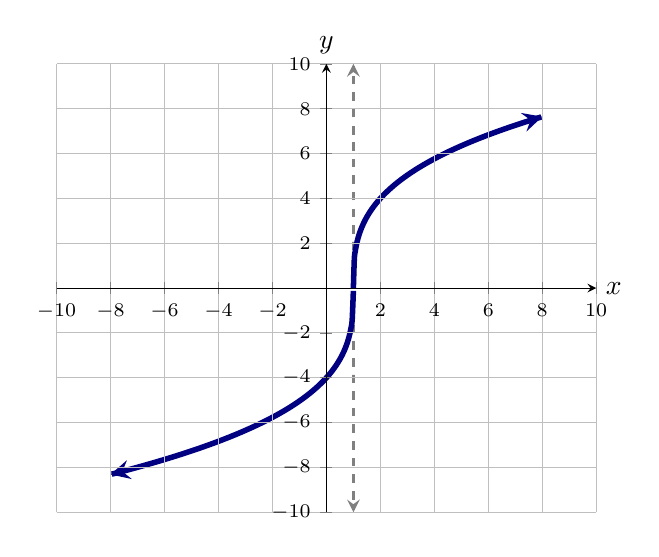
\begin{tikzpicture}
  \begin{axis}[
            domain=-10:10, ymax=10, xmax=10, ymin=-10, xmin=-10,
            axis lines =center, xlabel=$x$, ylabel=$y$, grid = major,
            ytick={-10,-8,-6,-4,-2,2,4,6,8,10},
            xtick={-10,-8,-6,-4,-2,2,4,6,8,10},
            ticklabel style={font=\scriptsize},
            every axis y label/.style={at=(current axis.above origin),anchor=south},
            every axis x label/.style={at=(current axis.right of origin),anchor=west},
            axis on top
          ]
          
			\addplot [line width=1, gray, dashed,samples=200,domain=(-10:10),<->] ({1},{x});
          	\addplot [line width=2, penColor, smooth,samples=200,domain=(-8:1),<-] {-4*((1-x)^0.333)};
          	\addplot [line width=2, penColor, smooth,samples=200,domain=(1:8),->] {4*((x-1)^0.333)};

          
            %\addplot [line width=1, gray, dashed,samples=200,domain=(-10:10),<->] ({x},{x});


          %\addplot[color=penColor,fill=penColor,only marks,mark=*] coordinates{(-2,-4)};


           

  \end{axis}
\end{tikzpicture}
\end{image}


This graph has a tangent line at $(1,0)$.  However, the tangent line is vertical, which means it doesn't have slope.  \\

Therefore, $f(1)$ does not exist.







\textbf{\textcolor{blue!55!black}{Corners:}} \\

There may not be a tangent line, like at a corner. \\
$f(x) = | x - 2 | - 3$ is an example.


\begin{image}
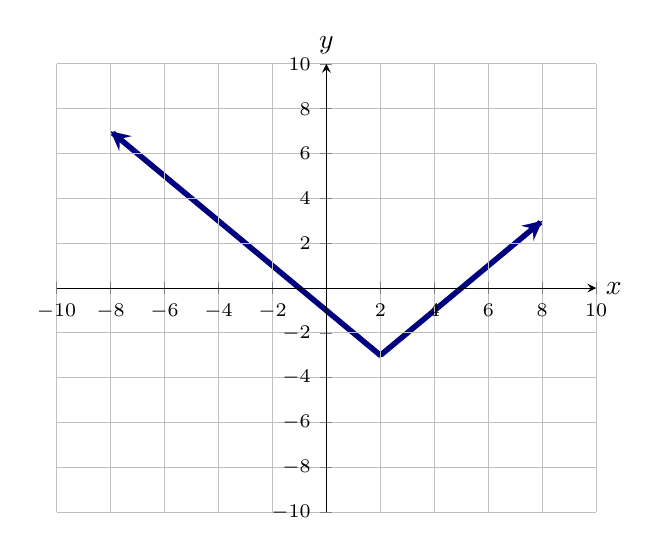
\begin{tikzpicture}
  \begin{axis}[
            domain=-10:10, ymax=10, xmax=10, ymin=-10, xmin=-10,
            axis lines =center, xlabel=$x$, ylabel=$y$, grid = major,
            ytick={-10,-8,-6,-4,-2,2,4,6,8,10},
            xtick={-10,-8,-6,-4,-2,2,4,6,8,10},
            ticklabel style={font=\scriptsize},
            every axis y label/.style={at=(current axis.above origin),anchor=south},
            every axis x label/.style={at=(current axis.right of origin),anchor=west},
            axis on top
          ]
          

          \addplot [line width=2, penColor, smooth,samples=200,domain=(-8:8),<->] {abs(x-2)-3};
          %\addplot [line width=2, penColor, smooth,samples=200,domain=(0:8),->] {4*((x-1)^0.333)};

          %\addplot [line width=1, gray, dashed,samples=200,domain=(-10:10),<->] ({1},{x});
            %\addplot [line width=1, gray, dashed,samples=200,domain=(-10:10),<->] ({x},{x});


          %\addplot[color=penColor,fill=penColor,only marks,mark=*] coordinates{(-2,-4)};


           

  \end{axis}
\end{tikzpicture}
\end{image}


This graph does not have a tangent line at $(2,-3)$.  When you approach $(2,-3)$ from the right or left, you get two different lines that describe the graph upon approaching.  They don't match. \\

Therefore, $f(2)$ does not exist.

















\textbf{\textcolor{blue!55!black}{Discontinuity:}} \\


There might be a discontinuity. \\
For example,


\[
f(x) = 
\begin{cases}
  -x &\text{if $x<-1$,}\\
  x-4 &\text{if $x\ge -1$}.
\end{cases}
\]


\begin{image}
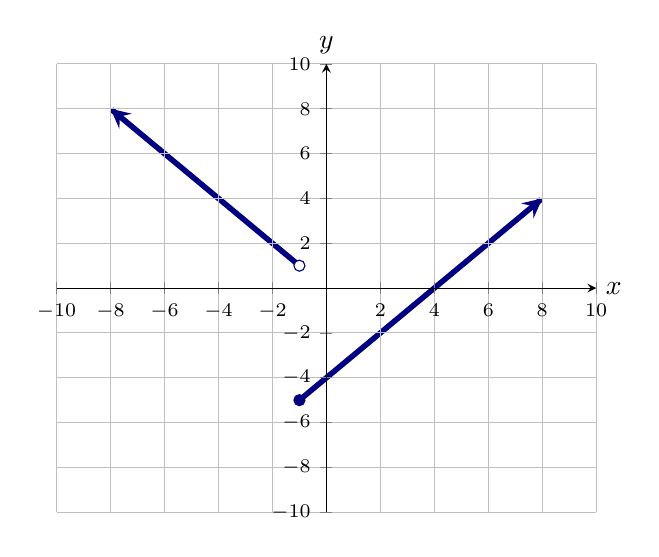
\begin{tikzpicture}
  \begin{axis}[
            domain=-10:10, ymax=10, xmax=10, ymin=-10, xmin=-10,
            axis lines =center, xlabel=$x$, ylabel=$y$, grid = major,
            ytick={-10,-8,-6,-4,-2,2,4,6,8,10},
            xtick={-10,-8,-6,-4,-2,2,4,6,8,10},
            ticklabel style={font=\scriptsize},
            every axis y label/.style={at=(current axis.above origin),anchor=south},
            every axis x label/.style={at=(current axis.right of origin),anchor=west},
            axis on top
          ]
          

          \addplot [line width=2, penColor, smooth,samples=200,domain=(-8:-1),<-] {-x};
          \addplot [line width=2, penColor, smooth,samples=200,domain=(-1:8),->] {x-4};
          %\addplot [line width=2, penColor, smooth,samples=200,domain=(0:8),->] {4*((x-1)^0.333)};

          %\addplot [line width=1, gray, dashed,samples=200,domain=(-10:10),<->] ({1},{x});
            %\addplot [line width=1, gray, dashed,samples=200,domain=(-10:10),<->] ({x},{x});


          \addplot[color=penColor,fill=penColor,only marks,mark=*] coordinates{(-1,-5)};
          \addplot[color=penColor,fill=white,only marks,mark=*] coordinates{(-1,1)};


           

  \end{axis}
\end{tikzpicture}
\end{image}


This graph does not have a tangent line at $(-1,-5)$.  When you approach $(-1,-5)$ from the right or left, you get two different lines that describe the graph upon approaching.  They don't match. \\

Therefore, $f(-1)$ does not exist. \\







\begin{idea} \textbf{\textcolor{green!50!black}{Critical Numbers}} \\



We use the derivative to establish a function's behavior: where a function is increasing or decreasing, or where local maximums and minimums occur.\\


Critical numbers are domain numbers where the derivative equals $0$ of does not exist. \\

Critical numbers are candidates for locations of maximums and minimums.


\end{idea}



However, there are other places where a function might exhibit a maximum or minimum. \\

For instances, at an endpoint. \\










\textbf{\textcolor{blue!55!black}{An Endpoint:}} \\


When we write our domains in reduced interval notation, the ends of our intervals might be included in the domain. These are not discontinuities, but they might be locations of extreme values of the function. \\


\[
f(x) = x-4 \, \text{ on } \, [-1, \infty)
\]


\begin{image}
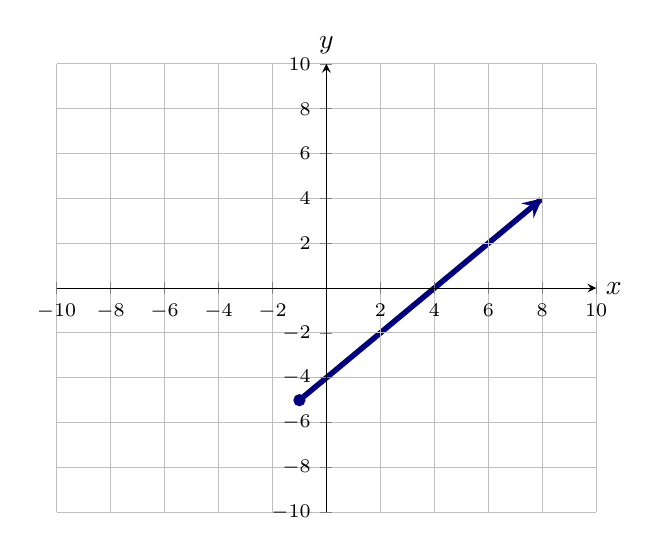
\begin{tikzpicture}
  \begin{axis}[
            domain=-10:10, ymax=10, xmax=10, ymin=-10, xmin=-10,
            axis lines =center, xlabel=$x$, ylabel=$y$, grid = major,
            ytick={-10,-8,-6,-4,-2,2,4,6,8,10},
            xtick={-10,-8,-6,-4,-2,2,4,6,8,10},
            ticklabel style={font=\scriptsize},
            every axis y label/.style={at=(current axis.above origin),anchor=south},
            every axis x label/.style={at=(current axis.right of origin),anchor=west},
            axis on top
          ]
          

          %\addplot [line width=2, penColor, smooth,samples=200,domain=(-8:-1),<-] {-x};
          \addplot [line width=2, penColor, smooth,samples=200,domain=(-1:8),->] {x-4};
          %\addplot [line width=2, penColor, smooth,samples=200,domain=(0:8),->] {4*((x-1)^0.333)};

          %\addplot [line width=1, gray, dashed,samples=200,domain=(-10:10),<->] ({1},{x});
            %\addplot [line width=1, gray, dashed,samples=200,domain=(-10:10),<->] ({x},{x});


          \addplot[color=penColor,fill=penColor,only marks,mark=*] coordinates{(-1,-5)};
          %\addplot[color=penColor,fill=white,only marks,mark=*] coordinates{(-1,1)};


           

  \end{axis}
\end{tikzpicture}
\end{image}


This graph has a tangent line at $(-1,-5)$.  \\

The line $y = x - 4$ is a tangent line to this graph at $(-1,-5)$ . \\

Therefore, $f(-1)$ exists and $f(-1) = 1$.  \\

$-1$ is not a critical number. \\


\begin{center}
\textbf{\textcolor{red!80!black}{We would prefer that $-1$ be a critical number for this function.}}
\end{center}














\subsection*{Revision}


With this example as motivation, we are going to revise our definition of the derivative. \\


We are going to force a little bit of space around $-1$ in the domain. \\




\begin{definition} \textbf{\textcolor{green!50!black}{Derivative}}  \\

Let $f(x)$ be a function with domain $D$. \\
Let $a \in D$ be a domain number. \\



For $f'(a)$ to exist, we need two things:

\begin{itemize}
\item There is an open interval inside the domain, which contains $a$.
\item The graph has a tangent line at $(a, f(a))$ and this tangent line has a slope.
\end{itemize}



\begin{center}

$f'(a)$ = the slope of the tangent line at $(a, f(a))$,

\end{center}



Otherwise, we say that $f'(a)$ does not exist (DNE).






\end{definition}


Now, endpoints can be critical numbers, because they do not have an open interval around them in the domain.  That automatically means the derivative does not exist there. \\






\begin{itemize}
\item This gives a more succinct way of talking about changing function behavior. 
\item This gives a more succinct way of talking about locations of extreme values. 
\end{itemize}




\begin{idea} \textbf{\textcolor{green!50!black}{Behavior}} \\


A function's behavior can change at \textbf{critical numbers} or \textbf{singularities}.






\end{idea}


\begin{example}


Suppose the function $g$ is defined on the domain $(-7, -1) \cup \{ 3 \} \cup (5, 10]$.

Then $3$ is automatically a critical number, because there is no open interval containing $3$ that is entirely inside the domain.\\


Singletons and endpoints are automatically critical numbers and candidates for locations of extreme values of function.


\end{example}



Calculus has further revisions.\\


Calculus will want more detail about endpoints.  Rather than just saying that they are critical numbers, Calculus will define left and right derivatives.  This will give us better ways to describe function behavior. \\













\begin{center}
\textbf{\textcolor{green!50!black}{ooooo-=-=-=-ooOoo-=-=-=-ooooo}} \\

more examples can be found by following this link\\ \link[More Examples of the Derivative]{https://ximera.osu.edu/csccmathematics/precalculus2/precalculus2/theDerivative/examples/exampleList}

\end{center}








\end{document}
